\documentclass[1p]{elsarticle_modified}
%\bibliographystyle{elsarticle-num}

%\usepackage[colorlinks]{hyperref}
%\usepackage{abbrmath_seonhwa} %\Abb, \Ascr, \Acal ,\Abf, \Afrak
\usepackage{amsfonts}
\usepackage{amssymb}
\usepackage{amsmath}
\usepackage{amsthm}
\usepackage{scalefnt}
\usepackage{amsbsy}
\usepackage{kotex}
\usepackage{caption}
\usepackage{subfig}
\usepackage{color}
\usepackage{graphicx}
\usepackage{xcolor} %% white, black, red, green, blue, cyan, magenta, yellow
\usepackage{float}
\usepackage{setspace}
\usepackage{hyperref}

\usepackage{tikz}
\usetikzlibrary{arrows}

\usepackage{multirow}
\usepackage{array} % fixed length table
\usepackage{hhline}

%%%%%%%%%%%%%%%%%%%%%
\makeatletter
\renewcommand*\env@matrix[1][\arraystretch]{%
	\edef\arraystretch{#1}%
	\hskip -\arraycolsep
	\let\@ifnextchar\new@ifnextchar
	\array{*\c@MaxMatrixCols c}}
\makeatother %https://tex.stackexchange.com/questions/14071/how-can-i-increase-the-line-spacing-in-a-matrix
%%%%%%%%%%%%%%%

\usepackage[normalem]{ulem}

\newcommand{\msout}[1]{\ifmmode\text{\sout{\ensuremath{#1}}}\else\sout{#1}\fi}
%SOURCE: \msout is \stkout macro in https://tex.stackexchange.com/questions/20609/strikeout-in-math-mode

\newcommand{\cancel}[1]{
	\ifmmode
	{\color{red}\msout{#1}}
	\else
	{\color{red}\sout{#1}}
	\fi
}

\newcommand{\add}[1]{
	{\color{blue}\uwave{#1}}
}

\newcommand{\replace}[2]{
	\ifmmode
	{\color{red}\msout{#1}}{\color{blue}\uwave{#2}}
	\else
	{\color{red}\sout{#1}}{\color{blue}\uwave{#2}}
	\fi
}

\newcommand{\Sol}{\mathcal{S}} %segment
\newcommand{\D}{D} %diagram
\newcommand{\A}{\mathcal{A}} %arc


%%%%%%%%%%%%%%%%%%%%%%%%%%%%%5 test

\def\sl{\operatorname{\textup{SL}}(2,\Cbb)}
\def\psl{\operatorname{\textup{PSL}}(2,\Cbb)}
\def\quan{\mkern 1mu \triangleright \mkern 1mu}

\theoremstyle{definition}
\newtheorem{thm}{Theorem}[section]
\newtheorem{prop}[thm]{Proposition}
\newtheorem{lem}[thm]{Lemma}
\newtheorem{ques}[thm]{Question}
\newtheorem{cor}[thm]{Corollary}
\newtheorem{defn}[thm]{Definition}
\newtheorem{exam}[thm]{Example}
\newtheorem{rmk}[thm]{Remark}
\newtheorem{alg}[thm]{Algorithm}

\newcommand{\I}{\sqrt{-1}}
\begin{document}

%\begin{frontmatter}
%
%\title{Boundary parabolic representations of knots up to 8 crossings}
%
%%% Group authors per affiliation:
%\author{Yunhi Cho} 
%\address{Department of Mathematics, University of Seoul, Seoul, Korea}
%\ead{yhcho@uos.ac.kr}
%
%
%\author{Seonhwa Kim} %\fnref{s_kim}}
%\address{Center for Geometry and Physics, Institute for Basic Science, Pohang, 37673, Korea}
%\ead{ryeona17@ibs.re.kr}
%
%\author{Hyuk Kim}
%\address{Department of Mathematical Sciences, Seoul National University, Seoul 08826, Korea}
%\ead{hyukkim@snu.ac.kr}
%
%\author{Seokbeom Yoon}
%\address{Department of Mathematical Sciences, Seoul National University, Seoul, 08826,  Korea}
%\ead{sbyoon15@snu.ac.kr}
%
%\begin{abstract}
%We find all boundary parabolic representation of knots up to 8 crossings.
%
%\end{abstract}
%\begin{keyword}
%    \MSC[2010] 57M25 
%\end{keyword}
%
%\end{frontmatter}

%\linenumbers
%\tableofcontents
%
\newcommand\colored[1]{\textcolor{white}{\rule[-0.35ex]{0.8em}{1.4ex}}\kern-0.8em\color{red} #1}%
%\newcommand\colored[1]{\textcolor{white}{ #1}\kern-2.17ex	\textcolor{white}{ #1}\kern-1.81ex	\textcolor{white}{ #1}\kern-2.15ex\color{red}#1	}

{\Large $\underline{11a_{119}~(K11a_{119})}$}

\setlength{\tabcolsep}{10pt}
\renewcommand{\arraystretch}{1.6}
\vspace{1cm}\begin{tabular}{m{100pt}>{\centering\arraybackslash}m{274pt}}
\multirow{5}{120pt}{
	\centering
	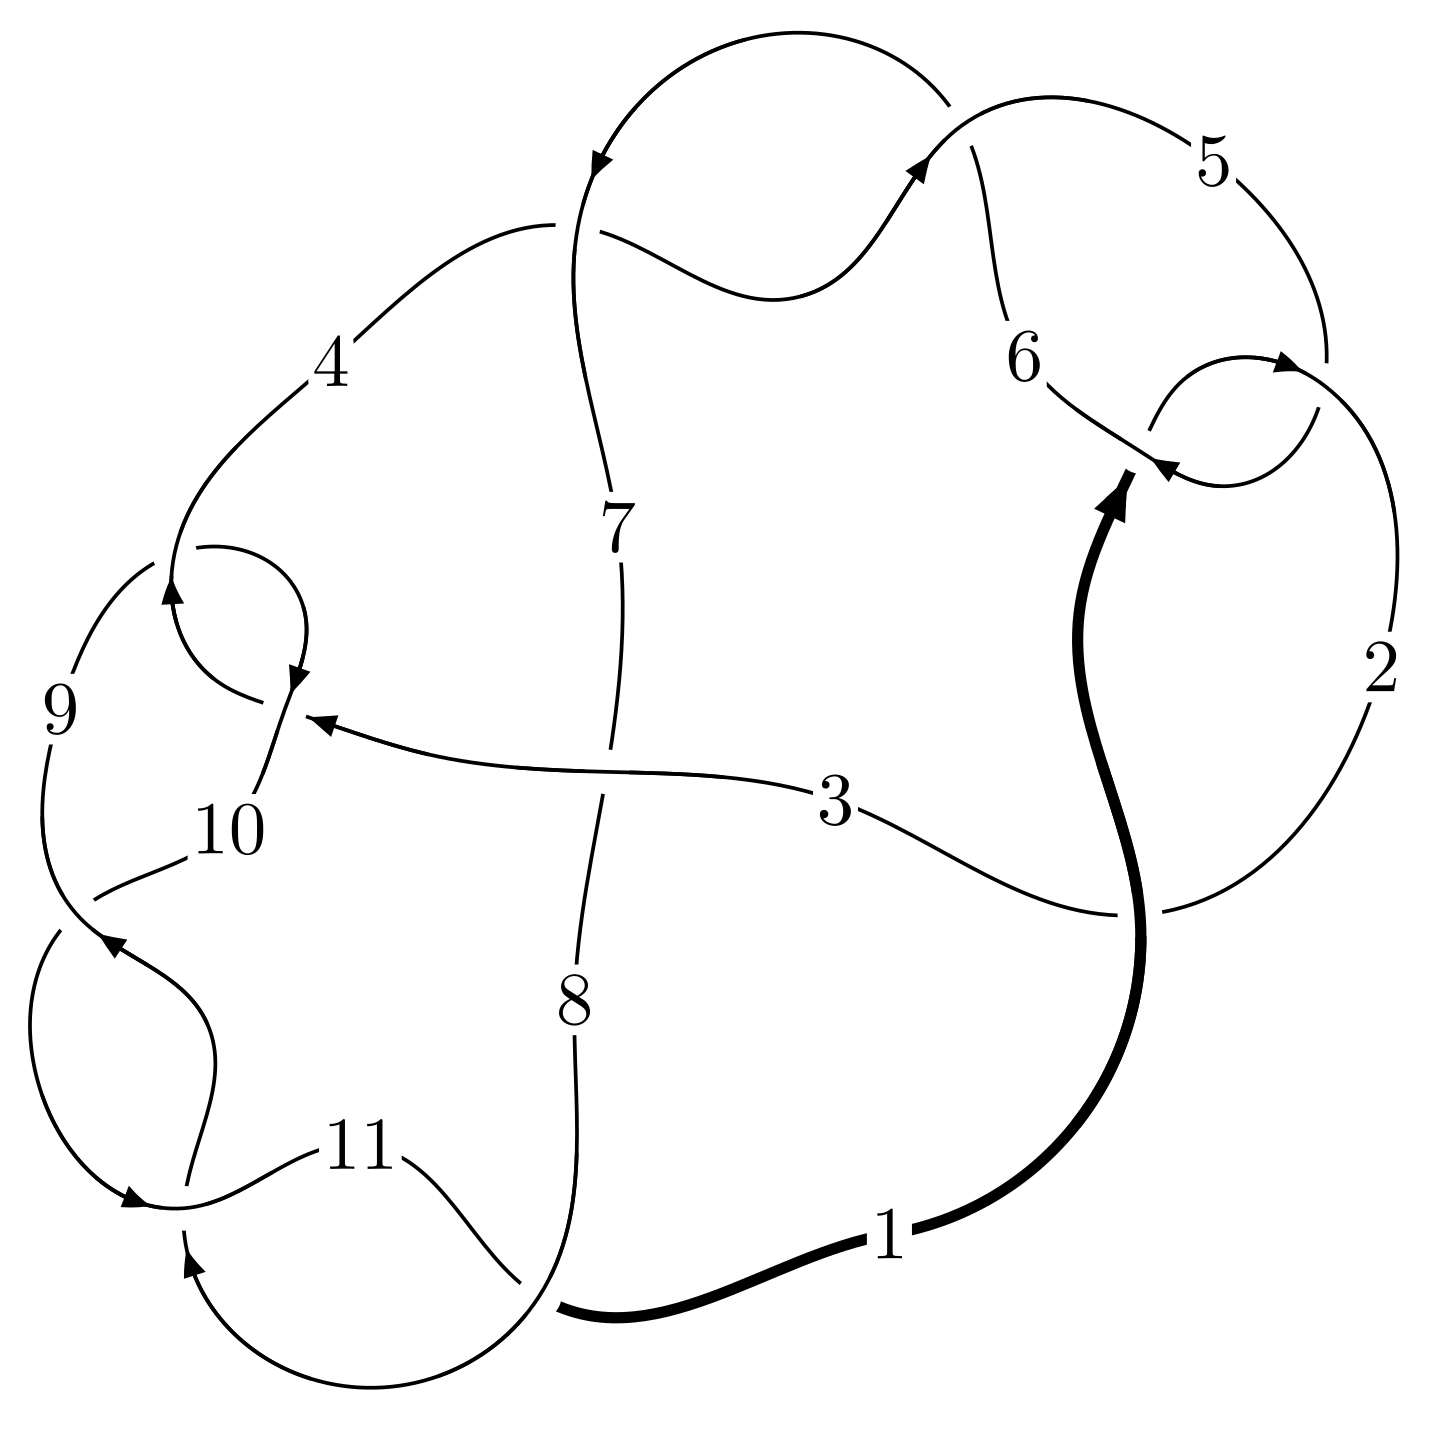
\includegraphics[width=112pt]{../../../GIT/diagram.site/Diagrams/png/368_11a_119.png}\\
\ \ \ A knot diagram\footnotemark}&
\allowdisplaybreaks
\textbf{Linearized knot diagam} \\
\cline{2-2}
 &
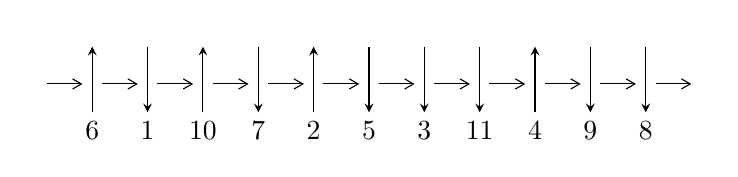
\begin{tikzpicture}[x=20pt, y=17pt]
	% nodes
	\node (C0) at (0, 0) {};
	\node (C1) at (1, 0) {};
	\node (C1U) at (1, +1) {};
	\node (C1D) at (1, -1) {6};

	\node (C2) at (2, 0) {};
	\node (C2U) at (2, +1) {};
	\node (C2D) at (2, -1) {1};

	\node (C3) at (3, 0) {};
	\node (C3U) at (3, +1) {};
	\node (C3D) at (3, -1) {10};

	\node (C4) at (4, 0) {};
	\node (C4U) at (4, +1) {};
	\node (C4D) at (4, -1) {7};

	\node (C5) at (5, 0) {};
	\node (C5U) at (5, +1) {};
	\node (C5D) at (5, -1) {2};

	\node (C6) at (6, 0) {};
	\node (C6U) at (6, +1) {};
	\node (C6D) at (6, -1) {5};

	\node (C7) at (7, 0) {};
	\node (C7U) at (7, +1) {};
	\node (C7D) at (7, -1) {3};

	\node (C8) at (8, 0) {};
	\node (C8U) at (8, +1) {};
	\node (C8D) at (8, -1) {11};

	\node (C9) at (9, 0) {};
	\node (C9U) at (9, +1) {};
	\node (C9D) at (9, -1) {4};

	\node (C10) at (10, 0) {};
	\node (C10U) at (10, +1) {};
	\node (C10D) at (10, -1) {9};

	\node (C11) at (11, 0) {};
	\node (C11U) at (11, +1) {};
	\node (C11D) at (11, -1) {8};
	\node (C12) at (12, 0) {};

	% arrows
	\draw[->,>={angle 60}]
	(C0) edge (C1) (C1) edge (C2) (C2) edge (C3) (C3) edge (C4) (C4) edge (C5) (C5) edge (C6) (C6) edge (C7) (C7) edge (C8) (C8) edge (C9) (C9) edge (C10) (C10) edge (C11) (C11) edge (C12) ;	\draw[->,>=stealth]
	(C1D) edge (C1U) (C2U) edge (C2D) (C3D) edge (C3U) (C4U) edge (C4D) (C5D) edge (C5U) (C6U) edge (C6D) (C7U) edge (C7D) (C8U) edge (C8D) (C9D) edge (C9U) (C10U) edge (C10D) (C11U) edge (C11D) ;
	\end{tikzpicture} \\
\hhline{~~} \\& 
\textbf{Solving Sequence} \\ \cline{2-2} 
 &
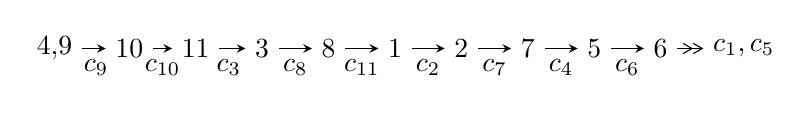
\begin{tikzpicture}[x=24pt, y=7pt]
	% node
	\node (A0) at (-1/8, 0) {4,9};
	\node (A1) at (1, 0) {10};
	\node (A2) at (2, 0) {11};
	\node (A3) at (3, 0) {3};
	\node (A4) at (4, 0) {8};
	\node (A5) at (5, 0) {1};
	\node (A6) at (6, 0) {2};
	\node (A7) at (7, 0) {7};
	\node (A8) at (8, 0) {5};
	\node (A9) at (9, 0) {6};
	\node (C1) at (1/2, -1) {$c_{9}$};
	\node (C2) at (3/2, -1) {$c_{10}$};
	\node (C3) at (5/2, -1) {$c_{3}$};
	\node (C4) at (7/2, -1) {$c_{8}$};
	\node (C5) at (9/2, -1) {$c_{11}$};
	\node (C6) at (11/2, -1) {$c_{2}$};
	\node (C7) at (13/2, -1) {$c_{7}$};
	\node (C8) at (15/2, -1) {$c_{4}$};
	\node (C9) at (17/2, -1) {$c_{6}$};
	\node (A10) at (41/4, 0) {$c_{1},c_{5}$};

	% edge
	\draw[->,>=stealth]	
	(A0) edge (A1) (A1) edge (A2) (A2) edge (A3) (A3) edge (A4) (A4) edge (A5) (A5) edge (A6) (A6) edge (A7) (A7) edge (A8) (A8) edge (A9) ;
	\draw[->>,>={angle 60}]	
	(A9) edge (A10);
\end{tikzpicture} \\ 

\end{tabular} \\

\footnotetext{
The image of knot diagram is generated by the software ``\textbf{Draw programme}" developed by Andrew Bartholomew(\url{http://www.layer8.co.uk/maths/draw/index.htm\#Running-draw}), where we modified some parts for our purpose(\url{https://github.com/CATsTAILs/LinksPainter}).
}\phantom \\ \newline 
\centering \textbf{Ideals for irreducible components\footnotemark of $X_{\text{par}}$} 
 
\begin{align*}
I^u_{1}&=\langle 
u^8+u^6+3 u^4+2 u^2- u+1\rangle \\
I^u_{2}&=\langle 
u^{30}- u^{29}+\cdots+2 u+1\rangle \\
\\
\end{align*}
\raggedright * 2 irreducible components of $\dim_{\mathbb{C}}=0$, with total 38 representations.\\
\footnotetext{All coefficients of polynomials are rational numbers. But the coefficients are sometimes approximated in decimal forms when there is not enough margin.}
\newpage
\renewcommand{\arraystretch}{1}
\centering \section*{I. $I^u_{1}= \langle u^8+u^6+3 u^4+2 u^2- u+1 \rangle$}
\flushleft \textbf{(i) Arc colorings}\\
\begin{tabular}{m{7pt} m{180pt} m{7pt} m{180pt} }
\flushright $a_{4}=$&$\begin{pmatrix}0\\u\end{pmatrix}$ \\
\flushright $a_{9}=$&$\begin{pmatrix}1\\0\end{pmatrix}$ \\
\flushright $a_{10}=$&$\begin{pmatrix}1\\- u^2\end{pmatrix}$ \\
\flushright $a_{11}=$&$\begin{pmatrix}u^2+1\\- u^2\end{pmatrix}$ \\
\flushright $a_{3}=$&$\begin{pmatrix}- u\\u^3+u\end{pmatrix}$ \\
\flushright $a_{8}=$&$\begin{pmatrix}u^4+u^2+1\\- u^4\end{pmatrix}$ \\
\flushright $a_{1}=$&$\begin{pmatrix}u^6+u^4+2 u^2+1\\- u^6- u^2\end{pmatrix}$ \\
\flushright $a_{2}=$&$\begin{pmatrix}- u^4- u^2-1\\u^6+2 u^4+u^3+2 u^2+1\end{pmatrix}$ \\
\flushright $a_{7}=$&$\begin{pmatrix}u\\u^6+u^4- u^3+2 u^2- u+1\end{pmatrix}$ \\
\flushright $a_{5}=$&$\begin{pmatrix}- u^3\\u^5+u^4+u^3+u^2+1\end{pmatrix}$ \\
\flushright $a_{6}=$&$\begin{pmatrix}u^5+u\\- u^7- u^5- u^3+u^2- u+1\end{pmatrix}$\\ \flushright $a_{6}=$&$\begin{pmatrix}u^5+u\\- u^7- u^5- u^3+u^2- u+1\end{pmatrix}$\\&\end{tabular}
\flushleft \textbf{(ii) Obstruction class $= -1$}\\~\\
\flushleft \textbf{(iii) Cusp Shapes $= -4 u^7-4 u^6-4 u^4-12 u^3-12 u^2-2$}\\~\\
\newpage\renewcommand{\arraystretch}{1}
\flushleft \textbf{(iv) u-Polynomials at the component}\newline \\
\begin{tabular}{m{50pt}|m{274pt}}
Crossings & \hspace{64pt}u-Polynomials at each crossing \\
\hline $$\begin{aligned}c_{1},c_{3},c_{5}\\c_{9}\end{aligned}$$&$\begin{aligned}
&u^8+u^6+3 u^4+2 u^2- u+1
\end{aligned}$\\
\hline $$\begin{aligned}c_{2},c_{4},c_{6}\\c_{8},c_{10},c_{11}\end{aligned}$$&$\begin{aligned}
&u^8+2 u^7+7 u^6+10 u^5+15 u^4+14 u^3+10 u^2+3 u+1
\end{aligned}$\\
\hline $$\begin{aligned}c_{7}\end{aligned}$$&$\begin{aligned}
&u^8-7 u^7+26 u^6-57 u^5+81 u^4-71 u^3+42 u^2-20 u+8
\end{aligned}$\\
\hline
\end{tabular}\\~\\
\newpage\renewcommand{\arraystretch}{1}
\flushleft \textbf{(v) Riley Polynomials at the component}\newline \\
\begin{tabular}{m{50pt}|m{274pt}}
Crossings & \hspace{64pt}Riley Polynomials at each crossing \\
\hline $$\begin{aligned}c_{1},c_{3},c_{5}\\c_{9}\end{aligned}$$&$\begin{aligned}
&y^8+2 y^7+7 y^6+10 y^5+15 y^4+14 y^3+10 y^2+3 y+1
\end{aligned}$\\
\hline $$\begin{aligned}c_{2},c_{4},c_{6}\\c_{8},c_{10},c_{11}\end{aligned}$$&$\begin{aligned}
&y^8+10 y^7+39 y^6+74 y^5+75 y^4+58 y^3+46 y^2+11 y+1
\end{aligned}$\\
\hline $$\begin{aligned}c_{7}\end{aligned}$$&$\begin{aligned}
&y^8+3 y^7+40 y^6+53 y^5+387 y^4-101 y^3+220 y^2+272 y+64
\end{aligned}$\\
\hline
\end{tabular}\\~\\
\newpage\flushleft \textbf{(vi) Complex Volumes and Cusp Shapes}
$$\begin{array}{c|c|c}  
\text{Solutions to }I^u_{1}& \I (\text{vol} + \sqrt{-1}CS) & \text{Cusp shape}\\
 \hline 
\begin{aligned}
u &= -0.338450 + 0.907350 I\end{aligned}
 & -2.36499 - 4.78635 I & -7.25990 + 9.32742 I \\ \hline\begin{aligned}
u &= -0.338450 - 0.907350 I\end{aligned}
 & -2.36499 + 4.78635 I & -7.25990 - 9.32742 I \\ \hline\begin{aligned}
u &= -0.894334 + 0.857566 I\end{aligned}
 & \phantom{-}13.66310 - 0.79369 I & \phantom{-}4.03459 + 2.11393 I \\ \hline\begin{aligned}
u &= -0.894334 - 0.857566 I\end{aligned}
 & \phantom{-}13.66310 + 0.79369 I & \phantom{-}4.03459 - 2.11393 I \\ \hline\begin{aligned}
u &= \phantom{-}0.840313 + 0.975020 I\end{aligned}
 & \phantom{-}12.9062 + 12.0580 I & \phantom{-}2.66730 - 7.52058 I \\ \hline\begin{aligned}
u &= \phantom{-}0.840313 - 0.975020 I\end{aligned}
 & \phantom{-}12.9062 - 12.0580 I & \phantom{-}2.66730 + 7.52058 I \\ \hline\begin{aligned}
u &= \phantom{-}0.392471 + 0.514949 I\end{aligned}
 & \phantom{-}0.469731 + 1.216760 I & \phantom{-}2.55801 - 5.53294 I \\ \hline\begin{aligned}
u &= \phantom{-}0.392471 - 0.514949 I\end{aligned}
 & \phantom{-}0.469731 - 1.216760 I & \phantom{-}2.55801 + 5.53294 I\\
 \hline 
 \end{array}$$\newpage\newpage\renewcommand{\arraystretch}{1}
\centering \section*{II. $I^u_{2}= \langle u^{30}- u^{29}+\cdots+2 u+1 \rangle$}
\flushleft \textbf{(i) Arc colorings}\\
\begin{tabular}{m{7pt} m{180pt} m{7pt} m{180pt} }
\flushright $a_{4}=$&$\begin{pmatrix}0\\u\end{pmatrix}$ \\
\flushright $a_{9}=$&$\begin{pmatrix}1\\0\end{pmatrix}$ \\
\flushright $a_{10}=$&$\begin{pmatrix}1\\- u^2\end{pmatrix}$ \\
\flushright $a_{11}=$&$\begin{pmatrix}u^2+1\\- u^2\end{pmatrix}$ \\
\flushright $a_{3}=$&$\begin{pmatrix}- u\\u^3+u\end{pmatrix}$ \\
\flushright $a_{8}=$&$\begin{pmatrix}u^4+u^2+1\\- u^4\end{pmatrix}$ \\
\flushright $a_{1}=$&$\begin{pmatrix}u^6+u^4+2 u^2+1\\- u^6- u^2\end{pmatrix}$ \\
\flushright $a_{2}=$&$\begin{pmatrix}u^{15}+2 u^{13}+6 u^{11}+8 u^9+10 u^7+8 u^5+4 u^3\\- u^{15}- u^{13}-4 u^{11}-3 u^9-4 u^7-2 u^5+u\end{pmatrix}$ \\
\flushright $a_{7}=$&$\begin{pmatrix}u^8+u^6+3 u^4+2 u^2+1\\- u^{10}-2 u^8-3 u^6-4 u^4- u^2\end{pmatrix}$ \\
\flushright $a_{5}=$&$\begin{pmatrix}- u^{17}-2 u^{15}-7 u^{13}-10 u^{11}-15 u^9-14 u^7-10 u^5-4 u^3- u\\u^{19}+3 u^{17}+8 u^{15}+15 u^{13}+19 u^{11}+21 u^9+14 u^7+6 u^5+u^3+u\end{pmatrix}$ \\
\flushright $a_{6}=$&$\begin{pmatrix}u^{26}+3 u^{24}+\cdots+3 u^2+1\\- u^{28}-4 u^{26}+\cdots-7 u^4-2 u^2\end{pmatrix}$\\ \flushright $a_{6}=$&$\begin{pmatrix}u^{26}+3 u^{24}+\cdots+3 u^2+1\\- u^{28}-4 u^{26}+\cdots-7 u^4-2 u^2\end{pmatrix}$\\&\end{tabular}
\flushleft \textbf{(ii) Obstruction class $= -1$}\\~\\
\flushleft \textbf{(iii) Cusp Shapes $= -4 u^{25}-12 u^{23}-44 u^{21}-88 u^{19}-4 u^{18}-164 u^{17}-12 u^{16}-224 u^{15}-32 u^{14}-256 u^{13}-56 u^{12}-228 u^{11}-72 u^{10}-160 u^9-72 u^8-88 u^7-48 u^6-40 u^5-20 u^4-28 u^3-4 u^2-12 u-6$}\\~\\
\newpage\renewcommand{\arraystretch}{1}
\flushleft \textbf{(iv) u-Polynomials at the component}\newline \\
\begin{tabular}{m{50pt}|m{274pt}}
Crossings & \hspace{64pt}u-Polynomials at each crossing \\
\hline $$\begin{aligned}c_{1},c_{3},c_{5}\\c_{9}\end{aligned}$$&$\begin{aligned}
&u^{30}- u^{29}+\cdots+2 u+1
\end{aligned}$\\
\hline $$\begin{aligned}c_{2},c_{4},c_{6}\\c_{8},c_{10},c_{11}\end{aligned}$$&$\begin{aligned}
&u^{30}+7 u^{29}+\cdots+4 u^2+1
\end{aligned}$\\
\hline $$\begin{aligned}c_{7}\end{aligned}$$&$\begin{aligned}
&(u^{15}+3 u^{14}+\cdots-5 u-7)^{2}
\end{aligned}$\\
\hline
\end{tabular}\\~\\
\newpage\renewcommand{\arraystretch}{1}
\flushleft \textbf{(v) Riley Polynomials at the component}\newline \\
\begin{tabular}{m{50pt}|m{274pt}}
Crossings & \hspace{64pt}Riley Polynomials at each crossing \\
\hline $$\begin{aligned}c_{1},c_{3},c_{5}\\c_{9}\end{aligned}$$&$\begin{aligned}
&y^{30}+7 y^{29}+\cdots+4 y^2+1
\end{aligned}$\\
\hline $$\begin{aligned}c_{2},c_{4},c_{6}\\c_{8},c_{10},c_{11}\end{aligned}$$&$\begin{aligned}
&y^{30}+31 y^{29}+\cdots+8 y+1
\end{aligned}$\\
\hline $$\begin{aligned}c_{7}\end{aligned}$$&$\begin{aligned}
&(y^{15}+9 y^{14}+\cdots-171 y-49)^{2}
\end{aligned}$\\
\hline
\end{tabular}\\~\\
\newpage\flushleft \textbf{(vi) Complex Volumes and Cusp Shapes}
$$\begin{array}{c|c|c}  
\text{Solutions to }I^u_{2}& \I (\text{vol} + \sqrt{-1}CS) & \text{Cusp shape}\\
 \hline 
\begin{aligned}
u &= \phantom{-}0.452252 + 0.939744 I\end{aligned}
 & \phantom{-}5.01187 + 2.09461 I & -0.30918 - 3.37423 I \\ \hline\begin{aligned}
u &= \phantom{-}0.452252 - 0.939744 I\end{aligned}
 & \phantom{-}5.01187 - 2.09461 I & -0.30918 + 3.37423 I \\ \hline\begin{aligned}
u &= -0.434887 + 0.955633 I\end{aligned}
 & \phantom{-}4.70557 - 8.28968 I & -1.16488 + 8.39094 I \\ \hline\begin{aligned}
u &= -0.434887 - 0.955633 I\end{aligned}
 & \phantom{-}4.70557 + 8.28968 I & -1.16488 - 8.39094 I \\ \hline\begin{aligned}
u &= -0.019728 + 0.944684 I\end{aligned}
 & \phantom{-}2.41074 + 3.00115 I & -4.85411 - 2.57684 I \\ \hline\begin{aligned}
u &= -0.019728 - 0.944684 I\end{aligned}
 & \phantom{-}2.41074 - 3.00115 I & -4.85411 + 2.57684 I \\ \hline\begin{aligned}
u &= -0.197860 + 0.871029 I\end{aligned}
 & -3.14864\phantom{ +0.000000I} & -11.00170 + 0. I\phantom{ +0.000000I} \\ \hline\begin{aligned}
u &= -0.197860 - 0.871029 I\end{aligned}
 & -3.14864\phantom{ +0.000000I} & -11.00170 + 0. I\phantom{ +0.000000I} \\ \hline\begin{aligned}
u &= \phantom{-}0.343092 + 0.793576 I\end{aligned}
 & -0.34244 + 1.73470 I & -0.36395 - 4.47971 I \\ \hline\begin{aligned}
u &= \phantom{-}0.343092 - 0.793576 I\end{aligned}
 & -0.34244 - 1.73470 I & -0.36395 + 4.47971 I \\ \hline\begin{aligned}
u &= \phantom{-}0.847869 + 0.850065 I\end{aligned}
 & \phantom{-}5.01187 - 2.09461 I & -0.30918 + 3.37423 I \\ \hline\begin{aligned}
u &= \phantom{-}0.847869 - 0.850065 I\end{aligned}
 & \phantom{-}5.01187 + 2.09461 I & -0.30918 - 3.37423 I \\ \hline\begin{aligned}
u &= \phantom{-}0.799403 + 0.896020 I\end{aligned}
 & \phantom{-}2.41074 + 3.00115 I & -4.85411 - 2.57684 I \\ \hline\begin{aligned}
u &= \phantom{-}0.799403 - 0.896020 I\end{aligned}
 & \phantom{-}2.41074 - 3.00115 I & -4.85411 + 2.57684 I \\ \hline\begin{aligned}
u &= -0.849380 + 0.882463 I\end{aligned}
 & \phantom{-}6.81987 - 1.98171 I & \phantom{-}4.04276 + 2.49548 I \\ \hline\begin{aligned}
u &= -0.849380 - 0.882463 I\end{aligned}
 & \phantom{-}6.81987 + 1.98171 I & \phantom{-}4.04276 - 2.49548 I \\ \hline\begin{aligned}
u &= \phantom{-}0.895044 + 0.849606 I\end{aligned}
 & \phantom{-}13.3047 - 5.6388 I & \phantom{-}3.41159 + 2.70946 I \\ \hline\begin{aligned}
u &= \phantom{-}0.895044 - 0.849606 I\end{aligned}
 & \phantom{-}13.3047 + 5.6388 I & \phantom{-}3.41159 - 2.70946 I \\ \hline\begin{aligned}
u &= \phantom{-}0.658622 + 0.369163 I\end{aligned}
 & \phantom{-}6.81987 + 1.98171 I & \phantom{-}4.04276 - 2.49548 I \\ \hline\begin{aligned}
u &= \phantom{-}0.658622 - 0.369163 I\end{aligned}
 & \phantom{-}6.81987 - 1.98171 I & \phantom{-}4.04276 + 2.49548 I \\ \hline\begin{aligned}
u &= -0.832514 + 0.928695 I\end{aligned}
 & \phantom{-}6.67502 - 4.27520 I & \phantom{-}3.73863 + 2.74888 I \\ \hline\begin{aligned}
u &= -0.832514 - 0.928695 I\end{aligned}
 & \phantom{-}6.67502 + 4.27520 I & \phantom{-}3.73863 - 2.74888 I \\ \hline\begin{aligned}
u &= \phantom{-}0.815148 + 0.948838 I\end{aligned}
 & \phantom{-}4.70557 + 8.28968 I & -1.16488 - 8.39094 I \\ \hline\begin{aligned}
u &= \phantom{-}0.815148 - 0.948838 I\end{aligned}
 & \phantom{-}4.70557 - 8.28968 I & -1.16488 + 8.39094 I \\ \hline\begin{aligned}
u &= -0.661870 + 0.335265 I\end{aligned}
 & \phantom{-}6.67502 + 4.27520 I & \phantom{-}3.73863 - 2.74888 I \\ \hline\begin{aligned}
u &= -0.661870 - 0.335265 I\end{aligned}
 & \phantom{-}6.67502 - 4.27520 I & \phantom{-}3.73863 + 2.74888 I \\ \hline\begin{aligned}
u &= -0.844833 + 0.970234 I\end{aligned}
 & \phantom{-}13.3047 - 5.6388 I & \phantom{-}3.41159 + 2.70946 I \\ \hline\begin{aligned}
u &= -0.844833 - 0.970234 I\end{aligned}
 & \phantom{-}13.3047 + 5.6388 I & \phantom{-}3.41159 - 2.70946 I \\ \hline\begin{aligned}
u &= -0.470358 + 0.199229 I\end{aligned}
 & -0.34244 + 1.73470 I & -0.36395 - 4.47971 I \\ \hline\begin{aligned}
u &= -0.470358 - 0.199229 I\end{aligned}
 & -0.34244 - 1.73470 I & -0.36395 + 4.47971 I\\
 \hline 
 \end{array}$$\newpage
\newpage\renewcommand{\arraystretch}{1}
\centering \section*{ III. u-Polynomials}
\begin{tabular}{m{50pt}|m{274pt}}
Crossings & \hspace{64pt}u-Polynomials at each crossing \\
\hline $$\begin{aligned}c_{1},c_{3},c_{5}\\c_{9}\end{aligned}$$&$\begin{aligned}
&(u^8+u^6+3 u^4+2 u^2- u+1)(u^{30}- u^{29}+\cdots+2 u+1)
\end{aligned}$\\
\hline $$\begin{aligned}c_{2},c_{4},c_{6}\\c_{8},c_{10},c_{11}\end{aligned}$$&$\begin{aligned}
&(u^8+2 u^7+7 u^6+10 u^5+15 u^4+14 u^3+10 u^2+3 u+1)\\
&\cdot(u^{30}+7 u^{29}+\cdots+4 u^2+1)
\end{aligned}$\\
\hline $$\begin{aligned}c_{7}\end{aligned}$$&$\begin{aligned}
&(u^8-7 u^7+26 u^6-57 u^5+81 u^4-71 u^3+42 u^2-20 u+8)\\
&\cdot(u^{15}+3 u^{14}+\cdots-5 u-7)^{2}
\end{aligned}$\\
\hline
\end{tabular}\newpage\renewcommand{\arraystretch}{1}
\centering \section*{ IV. Riley Polynomials}
\begin{tabular}{m{50pt}|m{274pt}}
Crossings & \hspace{64pt}Riley Polynomials at each crossing \\
\hline $$\begin{aligned}c_{1},c_{3},c_{5}\\c_{9}\end{aligned}$$&$\begin{aligned}
&(y^8+2 y^7+7 y^6+10 y^5+15 y^4+14 y^3+10 y^2+3 y+1)\\
&\cdot(y^{30}+7 y^{29}+\cdots+4 y^2+1)
\end{aligned}$\\
\hline $$\begin{aligned}c_{2},c_{4},c_{6}\\c_{8},c_{10},c_{11}\end{aligned}$$&$\begin{aligned}
&(y^8+10 y^7+39 y^6+74 y^5+75 y^4+58 y^3+46 y^2+11 y+1)\\
&\cdot(y^{30}+31 y^{29}+\cdots+8 y+1)
\end{aligned}$\\
\hline $$\begin{aligned}c_{7}\end{aligned}$$&$\begin{aligned}
&(y^8+3 y^7+40 y^6+53 y^5+387 y^4-101 y^3+220 y^2+272 y+64)\\
&\cdot(y^{15}+9 y^{14}+\cdots-171 y-49)^{2}
\end{aligned}$\\
\hline
\end{tabular}
\vskip 2pc
\end{document}